\documentclass[t]{beamer}
\usepackage{hyperref}
%\usepackage{french}
%\usepackage[latin1]{inputenc}
%\usepackage{times}
\usepackage[T1]{fontenc}
%\usepackage[a4paper]{geometry}

\definecolor{rrblitbackground}{rgb}{0.55, 0.3, 0.1}

\newenvironment{rtbliteral}{

\begin{ttfamily}

\color{rrblitbackground}

}{

\end{ttfamily}

}

\usetheme{Boadilla}

\setbeameroption{hide notes}

% generated by Docutils <http://docutils.sourceforge.net/>
\usepackage{cmap} % fix search and cut-and-paste in Acrobat
\usepackage{ifthen}
\usepackage[T1]{fontenc}
\usepackage[latin1]{inputenc}
\usepackage{graphicx}
\usepackage{alltt}

%%% Custom LaTeX preamble
% PDF Standard Fonts
\usepackage{mathptmx} % Times
\usepackage[scaled=.90]{helvet}
\usepackage{courier}

%%% User specified packages and stylesheets

%%% Fallback definitions for Docutils-specific commands

% class handling for environments (block-level elements)
% \begin{DUclass}{spam} tries \DUCLASSspam and
% \end{DUclass}{spam} tries \endDUCLASSspam
\ifx\DUclass\undefined % poor man's "provideenvironment"
 \newenvironment{DUclass}[1]%
  {\def\DocutilsClassFunctionName{DUCLASS#1}% arg cannot be used in end-part of environment.
     \csname \DocutilsClassFunctionName \endcsname}%
  {\csname end\DocutilsClassFunctionName \endcsname}%
\fi

% titlereference role
\providecommand*{\DUroletitlereference}[1]{\textsl{#1}}

% hyperlinks:
\ifthenelse{\isundefined{\hypersetup}}{
  \usepackage[colorlinks=true,linkcolor=blue,urlcolor=blue]{hyperref}
  \usepackage{bookmark}
  \urlstyle{same} % normal text font (alternatives: tt, rm, sf)
}{}
\hypersetup{
  pdftitle={Sage Combinat Widgets},
  pdfauthor={Odile B�nassy\{includegraphics\{images/logo-upsud\}\textbackslash{}The Author\}}
}

%%% Title Data
\title{\phantomsection%
  %
  \subtitle{A Quick Tour}
  \label{sage-combinat-widgets}}
\author{Odile B\'enassy}
\date{Feb.6, 2019 -- Combinatorics Seminar \@LIX}


%%% Body
\begin{document}

\begin{frame}[fragile]
\frametitle{Sage Combinat Widgets}


A collection of \textbf{interactive widgets} for the \emph{Jupyter} notebook
 \pause
\begin{itemize}

\item represent math objects
 \pause
\item graphically edit, and get the modified value
 \pause
\item can be used as building blocks in applications
 \pause
\item available for
\begin{itemize}

\item \footnotesize{(until now only grid-representable)} \normalsize{combinatorial objects}

\item \footnotesize{(until now only grid-representable)} \normalsize{graphs}

\item matrices
 \pause
\item \textbf{write your own}
\end{itemize}
\end{itemize}
\end{frame}

\begin{frame}[fragile]
\frametitle{Editing a Tableau (1)}

\begin{itemize}

\item edit/add/remove cells
\end{itemize}

\hspace{1cm}

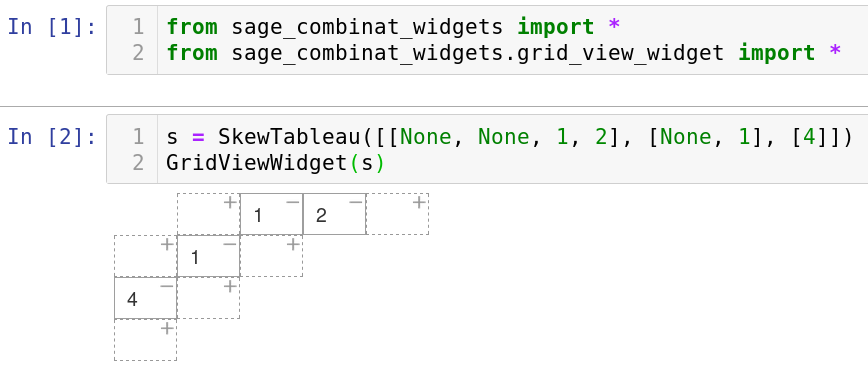
\includegraphics[scale=0.500000]{images/scrn-skewtableau}

\end{frame}

\begin{frame}[fragile]
\frametitle{Editing a Tableau (2)}

\begin{itemize}
\item \textquotedbl{}dirty\textquotedbl{} editing
\end{itemize}

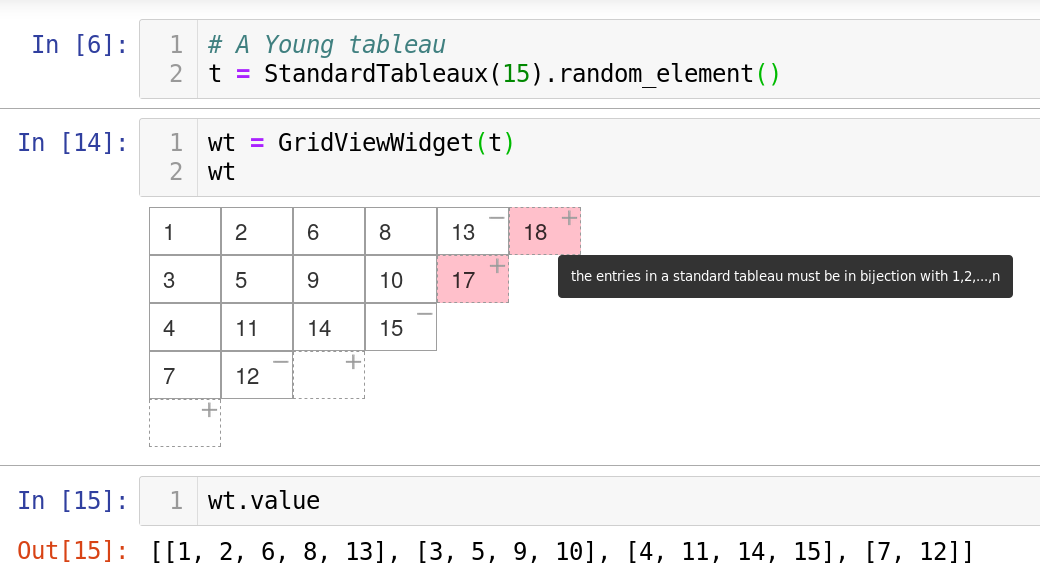
\includegraphics[scale=0.500000]{images/scrn-tableau}

\href{file:///home/odile/odk/sage/git/sage-combinat-widgets/docs/video/demo_youngtableau-short.ogv}{demo \#1}
\end{frame}

\begin{frame}[fragile]
\frametitle{Using @interact}

\begin{itemize}[<+-| alert@+>]

\item inserting a widget with \DUroletitlereference{@interact}
\end{itemize}

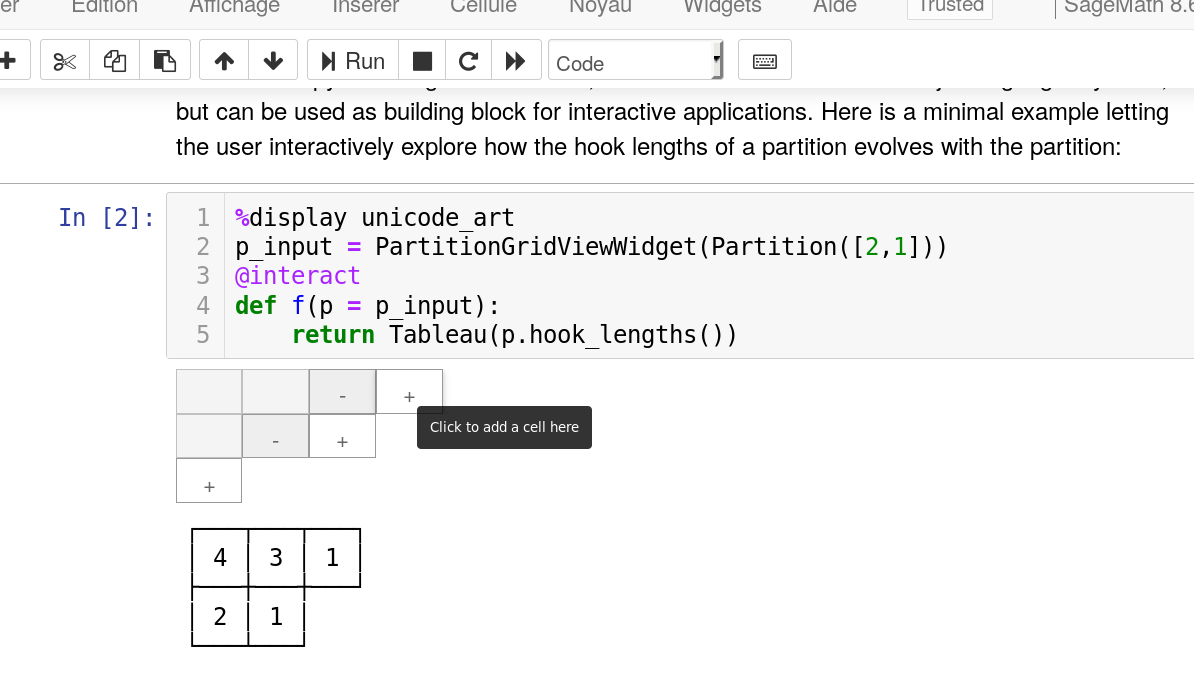
\includegraphics[scale=0.500000]{images/scrn-interact}

\href{file:///home/odile/odk/sage/git/sage-combinat-widgets/docs/video/demo_interact-short.ogv}{demo \#2}
\end{frame}

\begin{frame}[fragile]
\frametitle{Tossing Dominos}


\emph{an implementation of}
\url{http://images.math.cnrs.fr/Pavages-aleatoires-par-touillage}
\begin{columns}[T]
\column{0.47\textwidth}

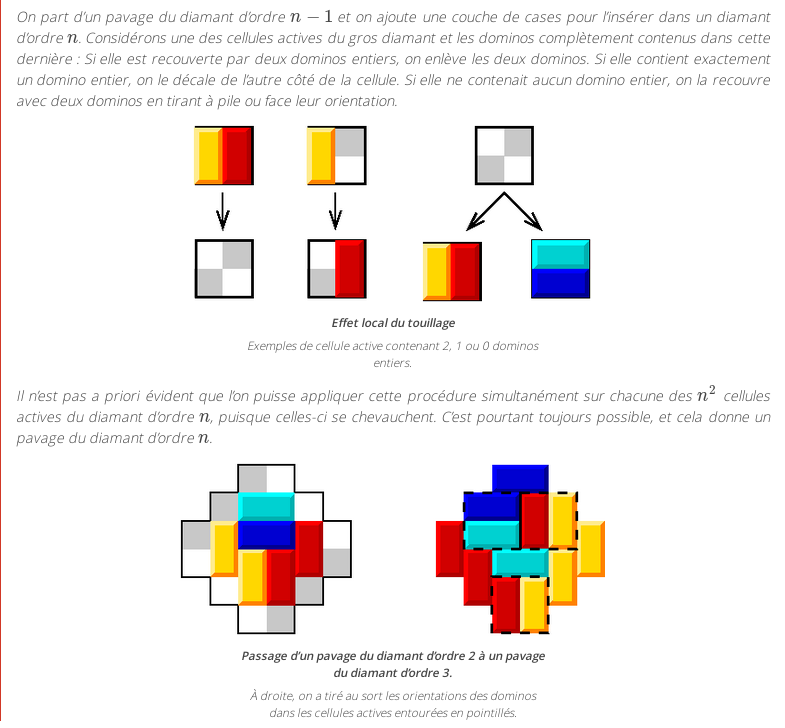
\includegraphics[scale=0.300000]{images/TossingAlgorithm}

\column{0.47\textwidth}

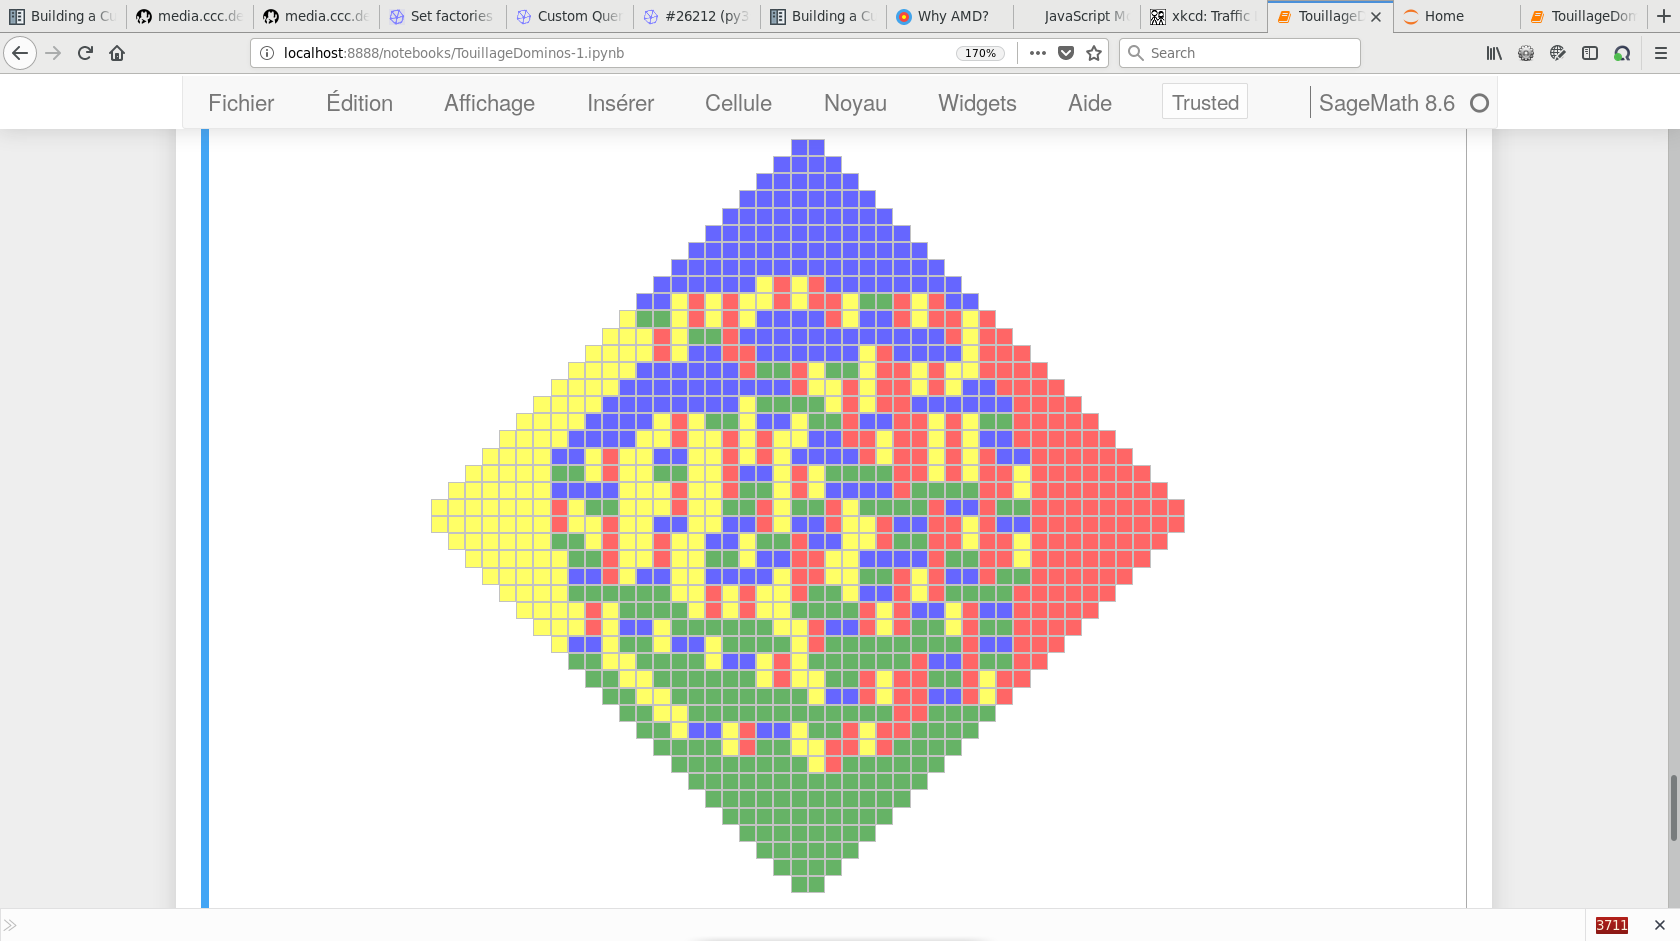
\includegraphics[scale=0.300000]{images/TossedDiamond22}

\end{columns}

\href{file:///home/odile/odk/sage/git/sage-combinat-widgets/docs/video/TossingDominos.ogv}{demo \#3}
\end{frame}

\begin{frame}[fragile]
\frametitle{Your own widget: Jeu de Taquin example (1)}


\emph{example based on}
\href{https://github.com/hivert/SageWidgetExper}{an experiment by Florent Hivert}

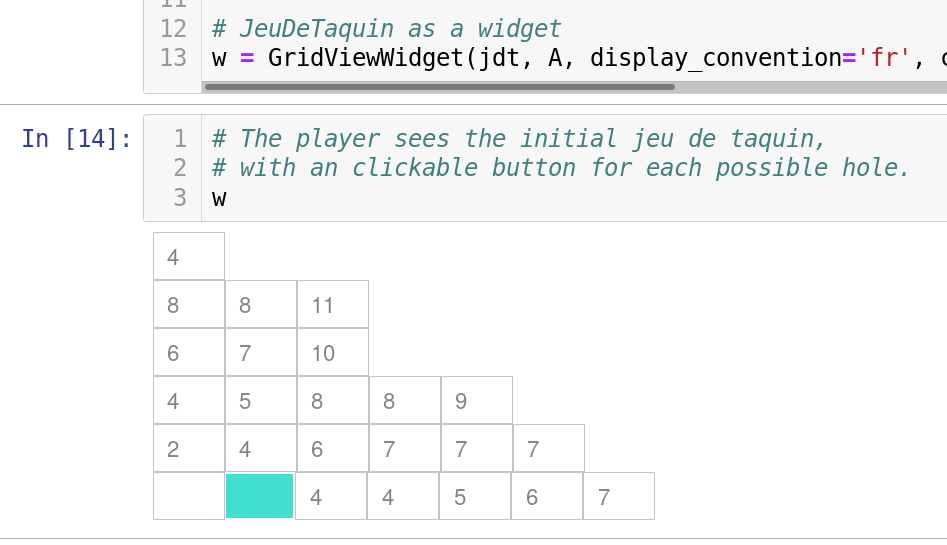
\includegraphics[scale=0.500000]{images/scrn-taquin}

\href{file:///home/odile/odk/sage/git/sage-combinat-widgets/docs/video/demo_taquin.ogv}{demo \#4}
\end{frame}

\begin{frame}[fragile]
\frametitle{Your own widget: Jeu de Taquin example (3)}

\begin{itemize}[<+-| alert@+>]

\item Math code \emph{(by F Hivert)}
\end{itemize}
\setbeamerfont{quote}{parent={}}

\begin{DUclass}{code-block}
\begin{quote}
\begin{alltt}
def create_hole(self, corner):
    /.../
    inner_corners = self.inner_shape().corners()
    if tuple(corner) not in inner_corners:
        raise ValueError("corner must be an inner corner")
    self._hole = corner
    self._new_st = self.to_list()
    spotl, spotc = self._hole
    self._new_st[spotl][spotc] = True

def slide(self):
    if self._hole is None:
        raise ValueError, "There is no hole"
    spotl, spotc = self._hole
    #Check to see if there is nothing to the right
    if spotc == len(self._new_st[spotl]) - 1:
        #Swap the hole with the cell below
        self._new_st[spotl][spotc] = self._new_st[spotl+1][spotc]
        self._new_st[spotl+1][spotc] = -1
        spotl += 1
    #Check to see if there is nothing below
    elif (spotl == len(self._new_st) - 1 or
          len(self._new_st[spotl+1]) <= spotc):
        #Swap the hole with the cell to the right
        /.../
\end{alltt}
\end{quote}
\end{DUclass}
\setbeamerfont{quote}{parent=quotation}
\end{frame}

\begin{frame}[fragile]
\frametitle{Your own widget: Jeu de Taquin example (3)}

\begin{itemize}[<+-| alert@+>]

\item Adapter source code
\end{itemize}
\setbeamerfont{quote}{parent={}}

\begin{DUclass}{code-block}
\begin{quote}
\begin{alltt}
# What happens when you click
@classmethod
def add_cell(cls, obj, pos, val, dirty=\{\}):
    # Create a hole if there isn't
    if not obj.has_hole():
        obj.create_hole(pos)
    # Slide
    obj.slide()
    return obj
\end{alltt}
\end{quote}
\end{DUclass}
\setbeamerfont{quote}{parent=quotation}
\end{frame}

\end{document}
